% !TEX root = domain_transduction.tex
Unsupervised domain adaptation is inherently a transduction problem since the main challenge lies in labeling the unsupervised data points with the help of the supervised data. Main complication is the domain shift between the supervised and unsupervised data points which makes existing transduction methods inapplicable. We explicitly model the domain shift and jointly solve for unsupervised labels as well as the domain shift in a fully transductive setup.

\subsection{Problem Definition}
In unsupervised domain adaptation problem, one of the domains is fully supervised $\{\xsi, \ysi \}_{i \in [N^s]}$ with $N^s$ data points $\xsi$ and corresponding labels $\ysi$ from a discrete set $\ysi \in \{1,\ldots, k \}$. Whereas, the other domain is unsupervised and only have $N^u$ data points $\{\xui \}_{i \in [N^u]}$. 


We further assume that both of the domains lie in the same space as $\xsi,\xui \in \mathcal{X}$ and there exist a feature function \mbox{$\Phi:\mathcal{X}\rightarrow \mathcal{R}^d$} which is applicable both of the domains. We separately study the case in which features function is a parametric function \mbox{$\Phi_\mathbf{\theta}:\mathcal{X}\rightarrow \mathcal{R}^d$} with a collection of parameters $\mathbf{\theta}$ to learn.

We explicitly model the domain shift in the form of a metric function and formulate our problem as a metric learning problem using an asymmetric similarity metric;
\begin{equation}
\sw(\xsi,\xuj) = \Phi(\xsi)^\intercal \mathbf{W} \Phi(\xuj)
\end{equation}
such that it is high if two data points $\xsj$ from the supervised and $\xui$ from the unsupervised domain are from the same class.

We model our learning setting in a fully transductive setting; in other words, the main purpose of the method is recovering the labels $\yui$ for each unsupervised example $\xui$. We consider the following objective function in order to compute $y_i$ as well as the similarity metric $\mathbf{W}$.

\begin{equation}
\begin{aligned}
\min_{\mathbf{W}, y_i} &\sum_{i \in [N^s]} &&[\sw(\xsi,\mathbf{x}_{i^-}) - \sw(\xsi,\mathbf{x}_{i^+}) + \alpha]_{+}  \\
&+\lambda &&\hspace{-3mm}\sum_{i \in N^u} \sum_{j \in \mathcal{N}(\xsi)}  \xui^\intercal \xuj \mathds{1}(y_i \neq y_j)\\
&s.t. \quad &&i^{+} = {\arg\max}_{j | y_j = \hat{y}_i} \sw(\mathbf{\hat{x}}_i,\mathbf{x}_{j}) \\
&\quad &&i^{-} = {\arg\max}_{j | y_j \neq \hat{y}_i} \sw(\mathbf{\hat{x}}_i,\mathbf{x}_{j}) 
\end{aligned}
\label{loss}
\end{equation}
where $\mathds{1}(a)$ is an indicator function which is $1$ if $a$ is true and $0$ otherwise and $[a]_+$ is a rectifier function which is equal to $\max(0, a)$. 

Our construction is based on the triplet loss defined in \cite{lmnn} with transduction extension. Original triplet loss \cite{lmnn} enforces a margin $\alpha$ for any data point between its similarity to the nearest neighbor from the same class and the nearest neighbor from other classes. We extend this construction to the unsupervised domain adaptation by enforcing a similar margin. For each supervised data point, we enforce a margin between its similarity to its nearest neighbors from the unsupervised data point having the same label and having a different label. We discuss this construction in detail in Section~\ref{metric}.

We further introduce a label consistency term in order to enforce consistency of the predicted labels of the unsupervised data points. In other words, we enforce that similar unsupervised data points should have the same label after the transduction. 



We solve this optimization problem via alternating minimization through iterating over solving for unsupervised labels $y_i$ and the similarity metric $\mathbf{W}$. We explain these two steps in detail in the following sections.

\subsection{Labeling Unsupervised Points}
\label{label}
\begin{figure}[ht]
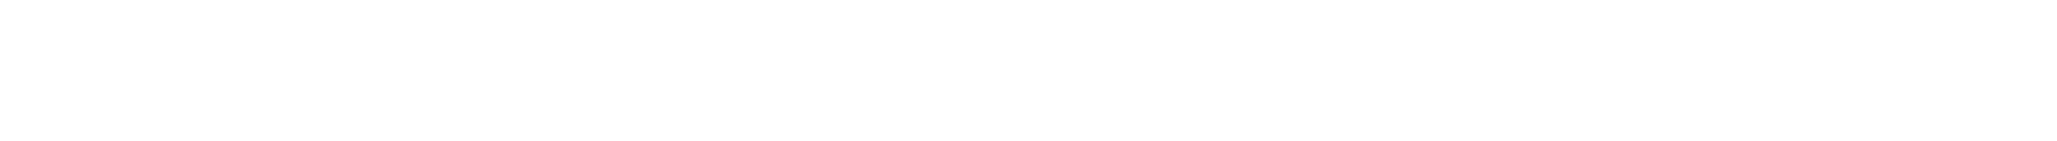
\includegraphics[width=\columnwidth]{figure1}
\caption{\textbf{Visualization of the Label Propogation.} Consider the unsupervised point $x_3$, the  resulting label would be:
\mbox{ ${\arg\min}_{y_3} -\sw(\hat{\mathbf{x}}_4,\mathbf{x}_3)\mathds{1}(\mathbf{y}_3=1) -\sw(\hat{\mathbf{x}}_{10},\mathbf{x}_3)\mathds{1}(y_3=2)$} $ -\sw(\hat{\mathbf{x}}_{11},\mathbf{x}_3)\mathds{1}(y_3=0) + \Phi(\mathbf{x}_2)^\intercal\phi(\mathbf{x}_3)\mathds{1}(y_3 \neq y_2) +\Phi(\mathbf{x}_3)^\intercal\phi(\mathbf{x}_4)\mathds{1}(y_3 \neq y_4) $ assuming green is $0$, blue is $1$ and red is $2$}
\label{vis_label_prop}
\end{figure}
In order to label the unsupervised data-points, we use nearest-neighbor(NN) rule. We simply compute the NN supervised datapoint for each unsupervised data point using the learned metric $\sw(\cdot,\cdot)$ and transfer the labels. In the initial stages of our optimization, our labeling needs to be accurate even with a sub-optimal similarity metric due to the iterative fashion of our algorithm. Hence, we enforce consistency of labels through label propagation. We first formally define the NN-rule and then introduce the label propagation.

Given a similarity metric $\sw(\cdot,\cdot)$, the nearest neighbor rule is;
\begin{equation}
(y_i)^{pred} = \hat{y}_{{\arg\max}_j \sw(\mathbf{x_i}, \mathbf{\hat{x}_j})}
\end{equation}

We use label propagation in order to enforce consistency of the predicted labels of unsupervised data points. Our label propagation construction is similar to existing graph transduction algorithms \cite{label_prop1,label_prop2}. In order to enforce this consistency, we create a k nearest neighbor (k-NN) graph over the unsupervised data points such that neighbor set $\mathcal{N}(\mathbf{x_i})$ for $\mathbf{x}_i$ is the k-unsupervised data point having highest similarity to $\mathbf{x_i}$ using the dot product in feature space. After the k-NN graph is created, we solve the following optimization problem for labeling unsupervised data points via label propogation;

\begin{equation}
\begin{aligned}
\min_{y_i}  &\sum_{i \in N^u}  \max_{\hat{y}_j=y_i}  \sw(\mathbf{\hat{x}_j},\mathbf{x}_{i}) \\
&+ \lambda
\sum_{i \in N^u} \sum_{j \in \mathcal{N}(\mathbf{x_i})} \mathbf{x}_i^T \mathbf{x}_j\mathds{1}(y_i \neq y_j)
\end{aligned}
\label{robtran}
\end{equation}

This problem can approximately be solved using many existing methods like $\alpha$-$\beta$ swapping, quadratic pseudo-boolean optimization (QPBO) and linear programming through roof-duality etc. We use $\alpha$-$\beta$ swapping algorithm from \cite{kolmogrovalphabeta} since it is experimentally shown to be efficient and accurate. Since it is rather out-of-scope of this paper, we explain the details of the $\alpha$-$\beta$ swapping algorithm in the appendix.

In order to further explain the label propagation, we visualize a sample example with $k=2$ and $3$-class classification problem in Figure~\ref{vis_label_prop}. 

It is also critical that this formulation requires solving high number of nearest neighbors and it is computationally challenging. However, our choice of optimization method and parameters makes this computation tractable. We use stochastic gradient descent with a carefully chosen batch size and only solve the NN over the examples in the batch. Furthermore, we also efficiently implement the distance computation using OpenBLAS as we further explain in detail in Section~\ref{imp_det}. 


\subsection{Learning the Similarity Metric}
\label{metric}
Given the predicted labels $y_i$ for unsupervised data points $\xui$, we need to learn an asymmetric metric in order to minimize the loss function defined in (\ref{loss}). 

The main intuition behind our formulation is to seek for a metric which can label the supervised data points correctly using the unsupervised data points and their predicted labels. In other words, we reverse the labeling direction. Since at this stage we already have a predicted label for each unsupervised data points, we can estimate a label for the supervised data points using these predicted labels. We also have ground truth labels for the supervised data points and we combine them to find a metric which will maximize the accuracy. In other words, the goal of the metric learning stage is;

\begin{itemize}
\item predicting $\hat{y}^{pred}_j$ using $\xui, \xsj, \ysj$
\item learning $\sw(\cdot,\cdot)$ by penalizing  $(\hat{y}_j)^{pred} \neq \hat{y}_j$ 
\end{itemize}

Fortunately, this can be jointly solved by minimizing the triplet loss as we define through supervised data points and the closest unsupervised data point of the same class as well as the closest unsupervised data point of a different class. Formally, we find the closest same class and different class unsupervised data points as;
\begin{equation}
\begin{aligned}
&i^{+} = {\arg\max}_{j | y_j = \hat{y}_i} \sw(\xsi, \xui) \\
&i^{-} = {\arg\max}_{j | y_j \neq \hat{y}_i} \sw(\xsi,\xuj) 
\label{sup_nn}
\end{aligned}
\end{equation}

We further define the loss function with regularizer using the nearest points as;
\begin{equation}
\min_{\mathbf{W}} \sum_{i \in [N^s]} [\sw(\mathbf{\hat{x_i}},\mathbf{x_{i^-}}) - \sw(\mathbf{\hat{x_i}},\mathbf{x_{i^+}}) + \alpha]_{+} + r(\mathbf{W})
\end{equation}
which is convex in terms of the $\mathbf{W}$ if the regularizer is convex; and we optimize it by using Stochastic gradient descent through the subgradient \
%\begin{small}
\mbox{$\frac{\partial loss (y_i, \mathbf{W})}{\partial \mathbf{W}} = \frac{\partial r ( \mathbf{W})}{\partial \mathbf{W}} + $}
\begin{equation}
\sum_{i \in [N^s]} \mathds{1}(\sw(\xsi,\mathbf{x_{i^-}}) - \sw(\xsi,\mathbf{x_{i^+}})>\alpha) \left( \xsi\mathbf{x}^\intercal_{i^-} - \xsi \mathbf{x}^\intercal_{i^+}  \right)  
\label{gradw}
\end{equation}
%\end{small}
As a regularizer we are using the Frobenius norm of the similarity matrix as $r(\mathbf{W})=\frac{1}{2}\|\mathbf{W}\|_F^2$. We explain the details of this optimization routine and how we implement in the Section~\ref{imp_det}.
\subsection{Learning Features}
In Section~\ref{label}~and~\ref{metric}, we developed our transductive labeling method with propogation as well as the metric learning algorithm using a pre-defined feature function $\Phi$. However, the current trends in machine learning suggests that learning this feature function $\Phi$ directly from the data  is a promising direction especially for visual domains. Hence, we consider the case $\Phi_{\mathbf{\theta}}$ is a parametrized feature function with parameter set $\mathbf{\theta}$. A typical example is CNNs(convolutional neural networks) with $\mathbf{\theta}$ as concatenation of weights and biases. We learn the feature function as part of the metric learning. In other words, during the metric learning stage, we also update the $\mathbf{\theta}$ using; $\frac{\partial loss (y_i, \mathbf{W})}{\partial \mathbf{\theta}} =$

\begin{small}
\begin{equation}
\begin{aligned}
 \sum_{i \in [N^s]} &\mathds{1}(\sw(\xsi,\mathbf{x_{i^-}}) - \sw(\xsi,\mathbf{x_{i^+}})>\alpha)  \\
 &\times \left(\frac{\partial \sw(\xsi,\mathbf{x_{i^-}}) }{\partial \mathbf{\Theta}} - \frac{\partial \sw(\xsi,\mathbf{x_{i^+}}) }{\partial \mathbf{\Theta}} \right)
 \label{gradt}
 \end{aligned}
\end{equation}
\end{small}
where $\frac{\partial \sw(\xsi,\xuj) }{\partial \mathbf{\Theta}} =\xuj^\intercal \mathbf{W} \frac{\partial \phi_\mathbf{\theta}(\xsi)}{\partial \theta} + \xsi^\intercal \mathbf{W} \frac{\partial \phi_\mathbf{\theta}(\xuj)}{\partial \theta} $

\begin{algorithm}[tb]
   \caption{Robust Transduction with Metric Learning}
   \label{alg:example}
\begin{algorithmic}
   \STATE {\bfseries Input:} unsupervised $\mathbf{x}_i$, supervised $\mathbf{\hat{x}}_i$, $y_i$, batch size $B$
   \REPEAT
   \STATE  Sample $(\mathbf{x}^b_1,\ldots \mathbf{x^b}_B)$, $(\mathbf{\hat{x}}^b_1,\ldots \mathbf{\hat{x}}^b_B)$, $(\hat{y}^b_1,\ldots \hat{x}^b_B)$
   \STATE Solve (\ref{robtran}) using $(\mathbf{x}^b_1,\ldots \mathbf{x^b}_B)$ and  $(\mathbf{\hat{x}}_1,\ldots \mathbf{\hat{x}}_{N^s})$
   \FOR{$i=1$ {\bfseries to} $B$}
      \IF{$ \hat{y}_i \textbf{ in } y_1 \ldots y_B $} 
   \STATE Compute ($i^+, i^-$) via $(\mathbf{x}^b_1,\ldots \mathbf{x^b}_B)$, $(\mathbf{\hat{x}}^b_1,\ldots \mathbf{\hat{x}}^b_B)$ 
   \STATE Update $\frac{\partial loss (y_i, \mathbf{W})}{\partial \mathbf{\Theta}}$ and  $\frac{\partial loss (y_i, \mathbf{W})}{\partial \mathbf{W}} $ using (\ref{gradw},\ref{gradt})
   \ENDIF
   \ENDFOR
   \STATE $\mathbf{W} \leftarrow \mathbf{W} + \alpha \frac{\partial loss (y_i, \mathbf{W})}{\partial \mathbf{W}}$ 
   \STATE $\mathbf{\Theta} \leftarrow \mathbf{\Theta} + \alpha \frac{\partial loss (y_i, \mathbf{W})}{\partial \mathbf{\Theta}}$
   \UNTIL CONVERGENCE or $MAX\_ITER$
\end{algorithmic}
\end{algorithm}

\subsection{Implementation Details}

\subsection{Weakly-Supervised Case}
